
\documentclass[10pt]{article}
\usepackage[utf8]{inputenc}
\usepackage{graphicx}
\usepackage{amsmath, amssymb}
\usepackage{geometry}
\usepackage{caption} 
\geometry{a4paper, margin=0.5in, landscape} 

\begin{document}

\section*{Comparative EIS Kinetics Report}
\textbf{Model Structure:} \texttt{R0-p(R1-p(R2-p(R3,CPE3),CPE2),CPE1)} \\
\textbf{Used data:} altered data, first 3 points removed and points with $freq > 2e+04$ removed

\begin{center}
    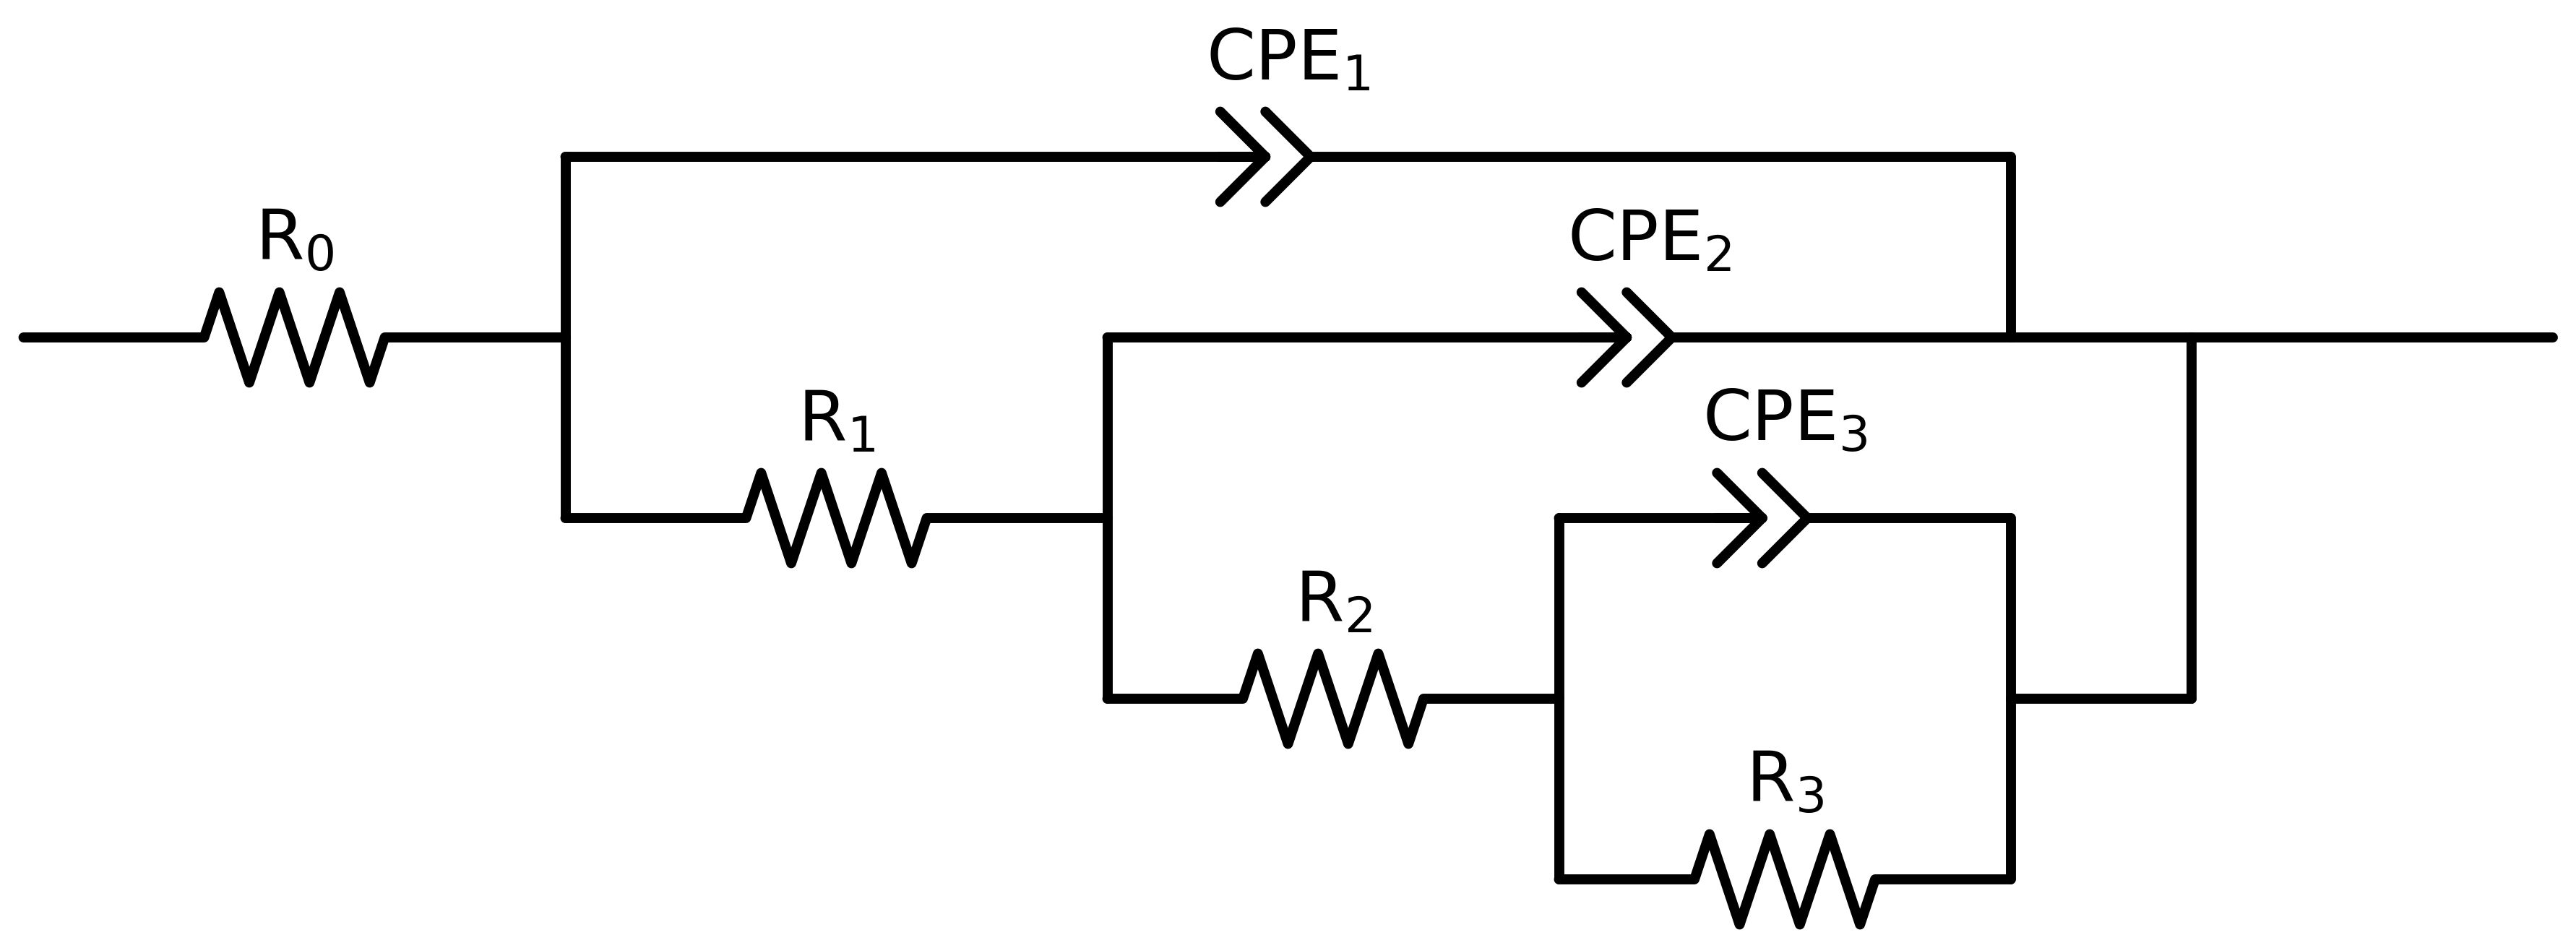
\includegraphics[width=0.45\textwidth]{../../3RC.png}
\end{center}

\renewcommand{\arraystretch}{1.6} 
\begin{table}[h!]
    \centering
    \footnotesize
    \begin{tabular}{|l|c|c|c|c|c|}
        \hline
        \textbf{Element} & \textbf{Unit} & \textbf{Bounds} & \textbf{Cauvel\_3\_BTA\_48H} & \textbf{Cauvel\_3\_BTA\_72H} & \textbf{Cauvel\_3\_BTA\_168H} \\ \hline
        $R_{0}$ & $\Omega$ & $[1.0e-03, 1.0e+03]$ & $8.31e+01 \pm 3.5e-01$ & $8.51e+01 \pm 3.7e-01$ & $8.55e+01 \pm 3.4e-01$ \\ \hline
        $R_{1}$ & $\Omega$ & $[1.0e+00, 1.0e+08]$ & $8.45e+03 \pm 4.9e+02$ & $1.42e+02 \pm 4.8e+01$ & $4.34e+03 \pm 5.4e+03$ \\ \hline
        $R_{2}$ & $\Omega$ & $[1.0e+00, 1.0e+08]$ & $1.93e+03 \pm 2.1e+03$ & $7.11e+03 \pm 1.7e+02$ & $1.00e+00 \pm 6.2e+03$ \\ \hline
        $R_{3}$ & $\Omega$ & $[1.0e+00, 1.0e+08]$ & $4.38e+04 \pm 2.1e+03$ & $3.49e+04 \pm 3.9e+02$ & $2.53e+04 \pm 4.8e+03$ \\ \hline
        $Q_{3}$ & $\Omega$$^{-1}$ sec$^{a}$ & $[1.0e-11, 1.0e-03]$ & $7.21e-06 \pm 1.7e-05$ & $3.85e-05 \pm 3.1e-07$ & $5.27e-05 \pm 1.8e-04$ \\ \hline
        $n_{3}$ & - & $[5.0e-01, 1.0e+00]$ & $5.00e-01 \pm 7.5e-01$ & $7.95e-01 \pm 6.7e-03$ & $8.67e-01 \pm 8.7e-01$ \\ \hline
        $Q_{2}$ & $\Omega$$^{-1}$ sec$^{a}$ & $[1.0e-11, 1.0e-03]$ & $1.73e-05 \pm 1.7e-05$ & $8.88e-07 \pm 4.6e-07$ & $3.16e-05 \pm 2.0e-04$ \\ \hline
        $n_{2}$ & - & $[5.0e-01, 1.0e+00]$ & $9.14e-01 \pm 2.0e-01$ & $9.89e-01 \pm 4.6e-02$ & $5.00e-01 \pm 1.2e+00$ \\ \hline
        $Q_{1}$ & $\Omega$$^{-1}$ sec$^{a}$ & $[1.0e-11, 1.0e-03]$ & $1.15e-05 \pm 2.3e-07$ & $9.81e-06 \pm 7.6e-07$ & $1.12e-05 \pm 3.9e-07$ \\ \hline
        $n_{1}$ & - & $[5.0e-01, 1.0e+00]$ & $8.64e-01 \pm 2.9e-03$ & $8.54e-01 \pm 6.0e-03$ & $8.64e-01 \pm 4.5e-03$ \\ \hline
        \textbf{$\chi^2$} & - & -  & $1.828e-04$ & $7.848e-05$ & $1.517e-04$ \\ \hline

    \end{tabular}
\end{table}


\newpage
\section*{Analysis Results: 48H}
\begin{center}
    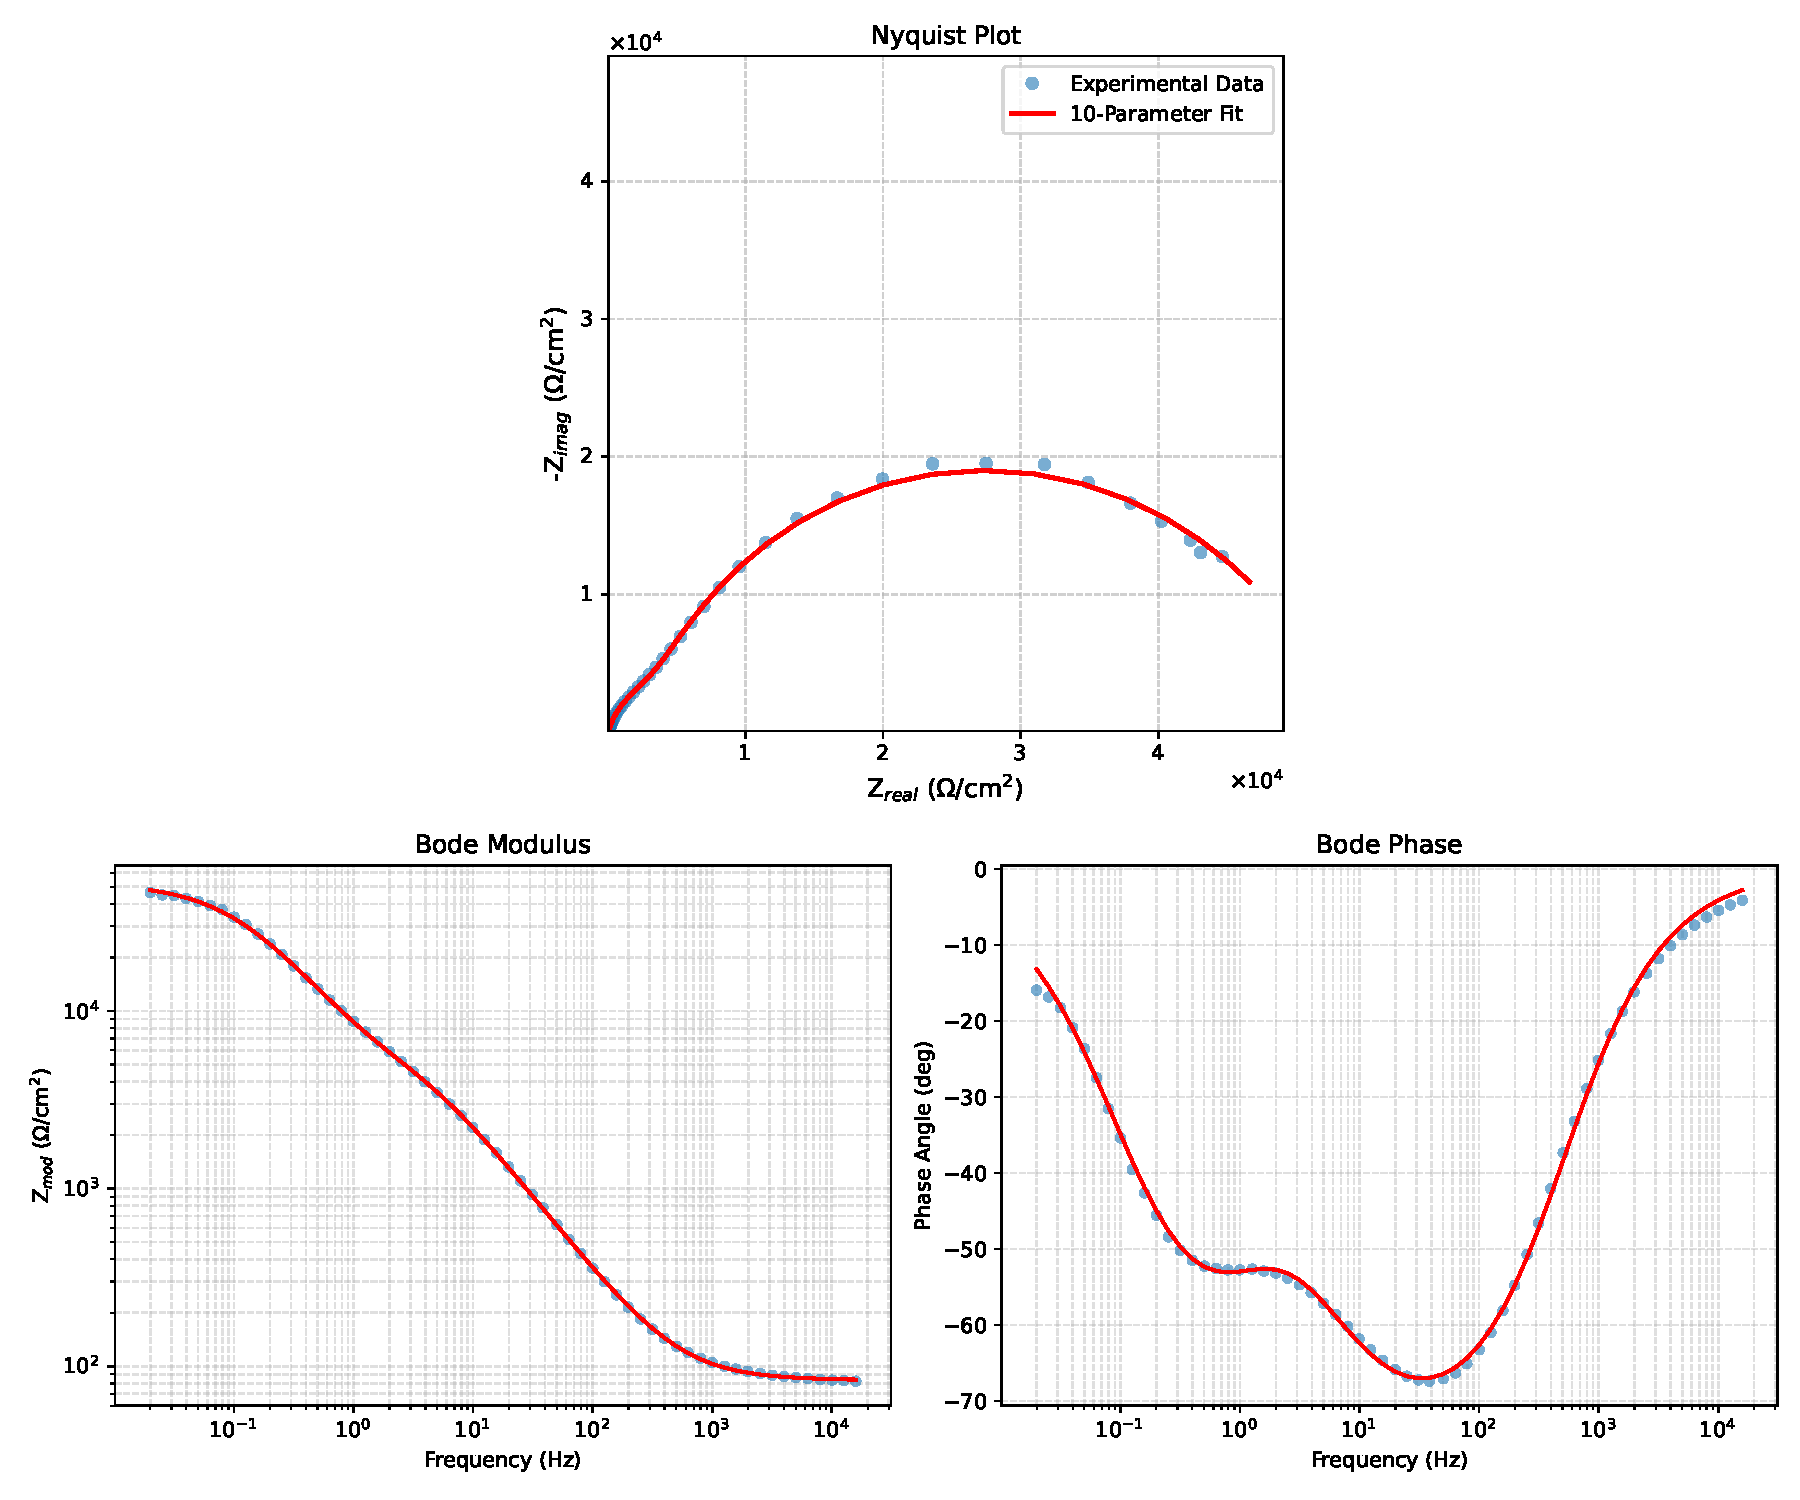
\includegraphics[width=0.7\textwidth]{plots_Cauvel_3_BTA_48H_3RC.pdf}
    \captionof{figure}{EIS Fit Results for Cauvel\_3\_BTA\_48H}
\end{center}

\newpage
\section*{Analysis Results: 72H}
\begin{center}
    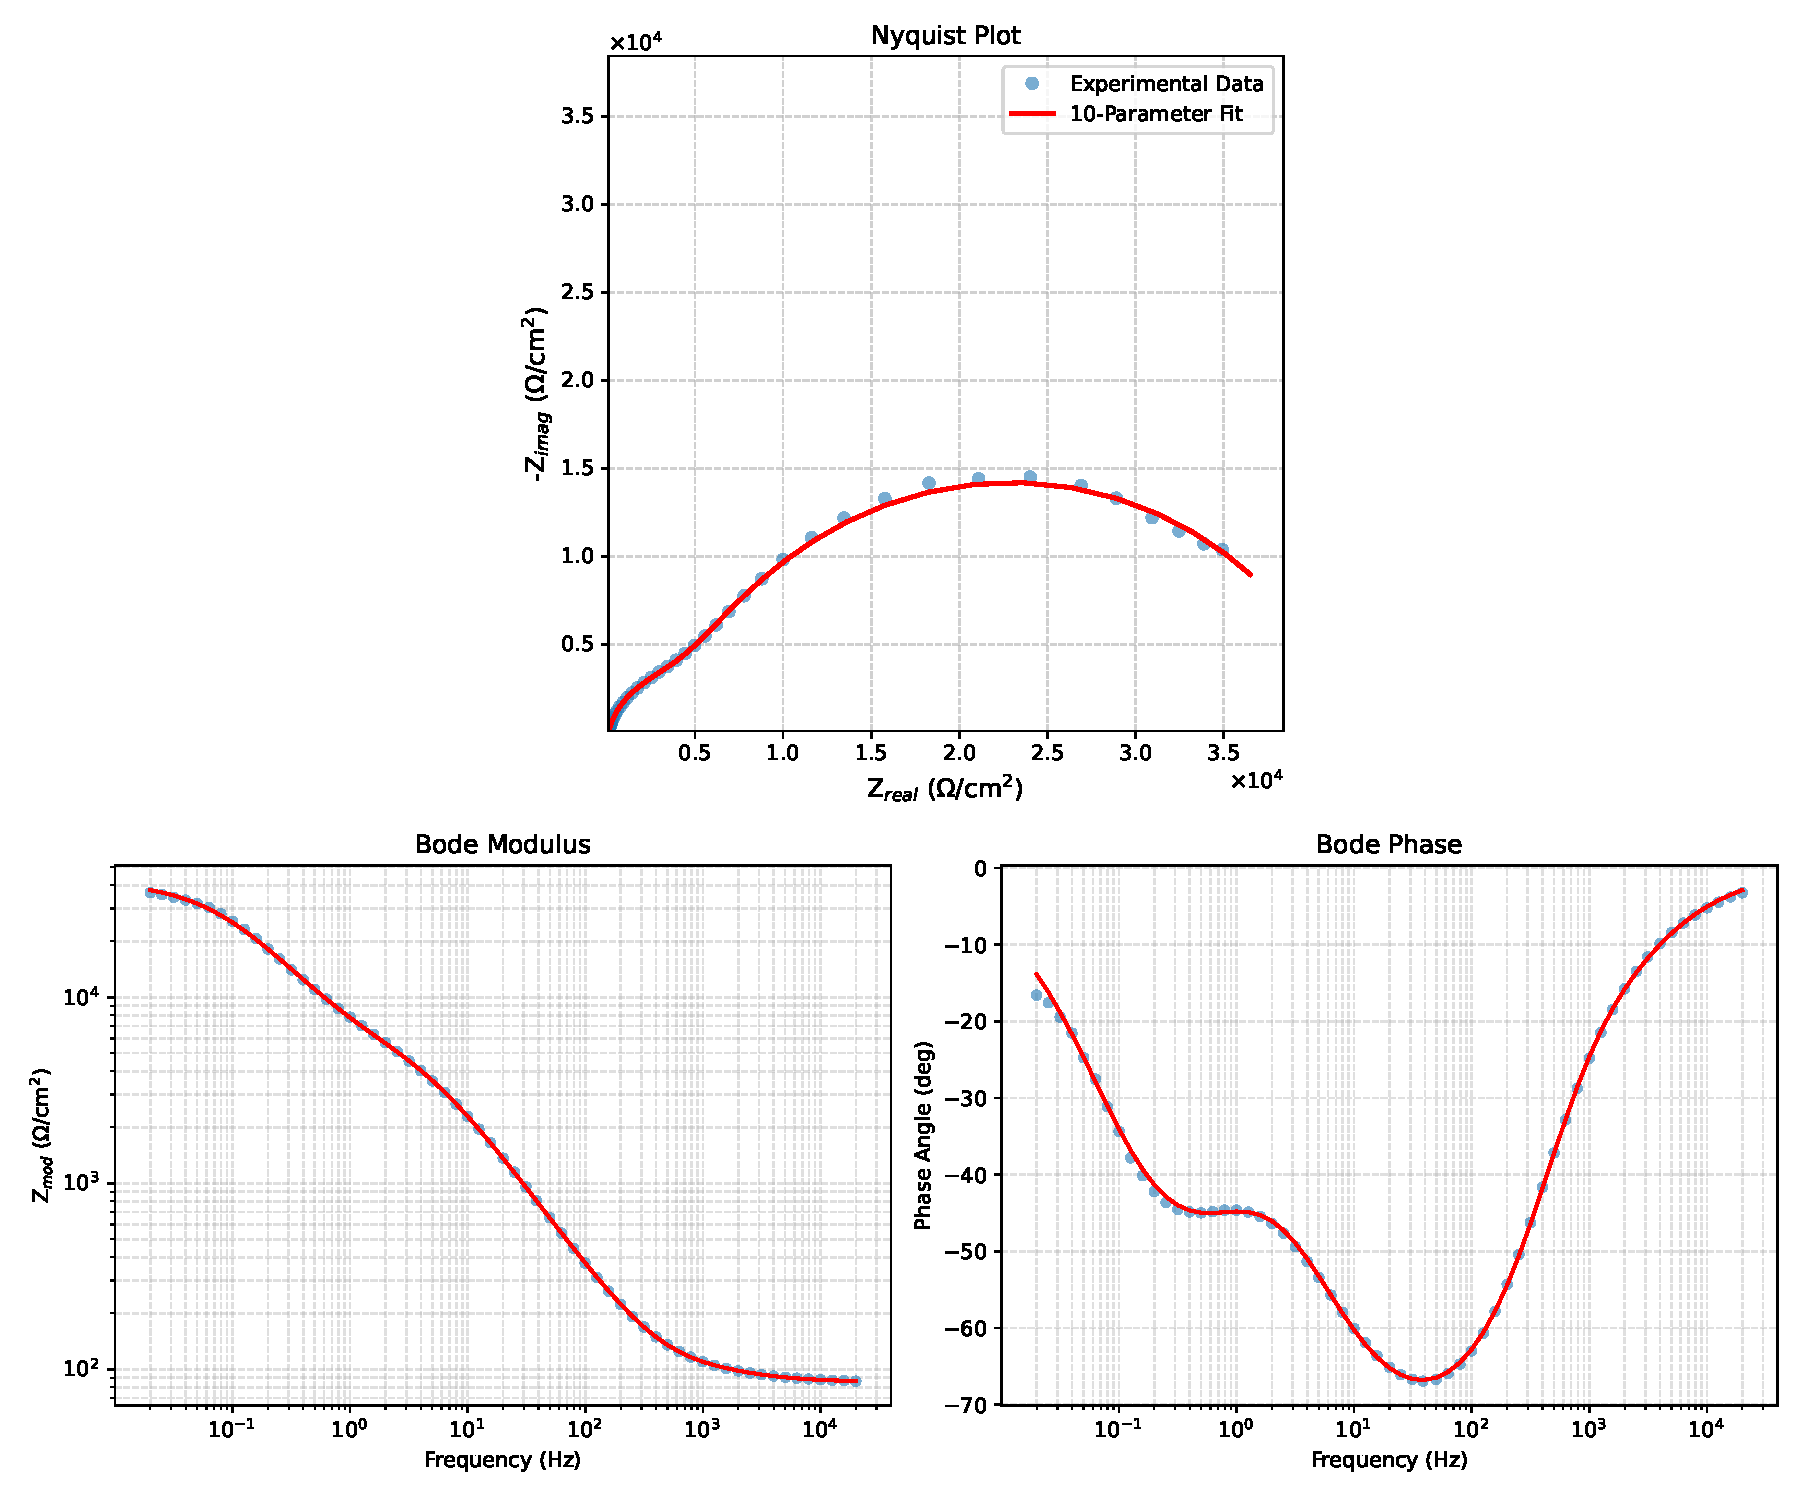
\includegraphics[width=0.7\textwidth]{plots_Cauvel_3_BTA_72H_3RC.pdf}
    \captionof{figure}{EIS Fit Results for Cauvel\_3\_BTA\_72H}
\end{center}

\newpage
\section*{Analysis Results: 168H}
\begin{center}
    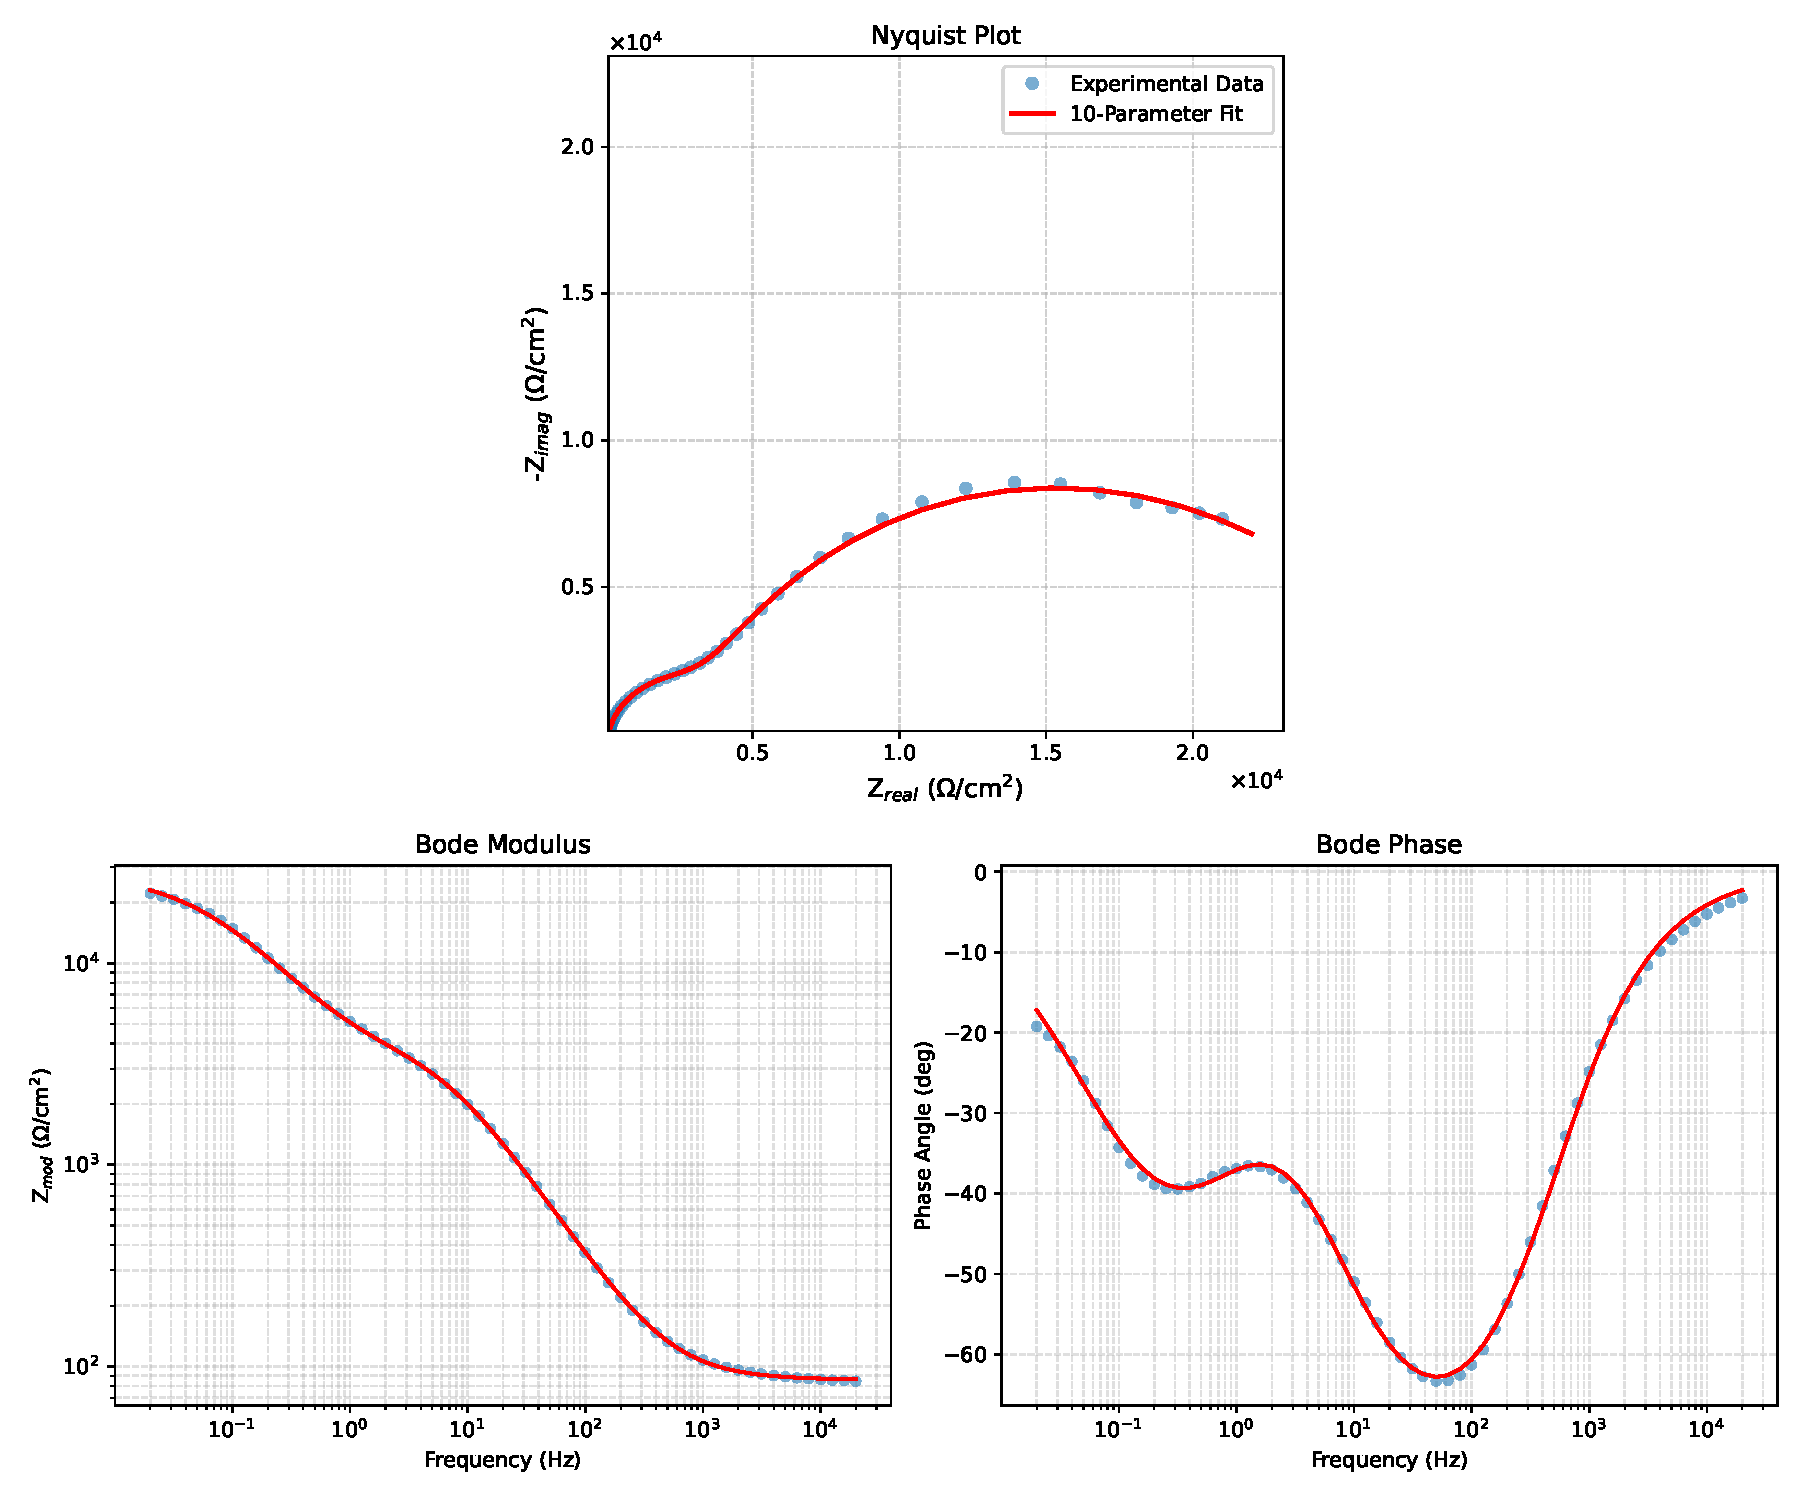
\includegraphics[width=0.7\textwidth]{plots_Cauvel_3_BTA_168H_3RC.pdf}
    \captionof{figure}{EIS Fit Results for Cauvel\_3\_BTA\_168H}
\end{center}


\end{document}
